\section{The New Algorithms}
\label{sec:algorithms}
%\vspace{-6pt}
We describe in this section new algorithms that overcome the shortcomings mentioned earlier; 
the new algorithms use additional pruning strategies, maintain simplicity, and 
avoid a sequential computational order.
We begin by first introducing the following notations.
%Let $G = (V,E)$ denote a simple undirected graph, and let $n = \left|V\right|$ and $m = \left|E\right|$. 
We identify the $n$ vertices of the input graph $G=(V,E)$ as $\{v_1, v_2, \ldots, v_n\}$.  
The set of vertices adjacent to a vertex $v_i$, the set of its neighbors, is denoted by $N(v_i)$.
And the degree of the vertex $v_i$, the cardinality of $N(v_i)$, is 
denoted by $d(v_i)$.  

%\vspace{-10pt}
\subsection{The Exact Algorithm}
\label{subsec:exact}
%\vspace{-4pt}

Recall that the maximum clique in a graph can be found by computing the largest clique containing each vertex and picking the largest among these. 
A key element of our exact algorithm is that during the search for the largest clique containing a given vertex, vertices that cannot form cliques larger than the current maximum 
clique are {\em pruned}, in a hierarchical fashion. 
The method is outlined in detail in Algorithm \ref{alg:mClq}. 
Throughout, the variable $max$ stores the size of the maximum clique found 
thus far. Initially it is set to be equal to the lower bound $lb$ provided as an input parameter.
It gives the maximum clique size when the algorithm terminates.

\begin{figure}
%\vspace{14pt}
\hrule
\vspace{6pt}
\begin{spacing}{\algospacing}
{
{\small
\captionof{algorithm}{{\protect\small Algorithm for finding the maximum clique of a given graph.
{\it Input}: Graph $G = \left (V, E\right )$, lower bound on clique $lb$ (default, 0). {\it Output}: Size of maximum clique.}}\label{alg:mClq}
\vspace{-5pt}
\hrule
\vspace{6pt}

\noindent\begin{minipage}{.5\textwidth}
\vspace{-12pt}
\begin{algorithmic}[1]
\Procedure {MaxClique}{$G=\left (V,E\right )$, $lb$}
\State $max \leftarrow lb$
\For{$i:1$ to $n$}
%\If{$degree(v_i) < maxClq$} 
%\State continue \Comment{{\small Pruning 1}}
%\EndIf
\If{$d(v_i) \ge max$} \Comment{{\footnotesize Pruning 1}} \label{pr1}
\State $U \leftarrow \emptyset$
\For{each $v_j \in N(v_i)$}
\If{$j > i$} \Comment{{\footnotesize Pruning 2}} \label{prOld}
\If{$d(v_j) \ge max$} \Comment{{\footnotesize Pruning 3}} \label{pr2}
\State $U \leftarrow U \cup \{v_j\}$ 
\EndIf
\EndIf
\EndFor

\State \textsc{Clique}$(G, U, 1)$ \label{subCall}
\EndIf

\EndFor
\EndProcedure
\end{algorithmic}
\end{minipage}%
\begin{minipage}{.5\textwidth}
\captionof*{algorithm}{{\em Subroutine}}
\vspace{-6pt}
\begin{algorithmic}[1]
\Procedure {Clique}{$G=\left (V,E\right )$, $U$, $size$}

\If{$U = \emptyset$}
\If{$size > max$} 
\State $max \leftarrow size$ \label{critical}
\EndIf
\State {\bf return}
\EndIf

\While{$\left|U\right| > 0$}
\If{$size + \left|{U}\right| \le max$} \Comment{{\footnotesize Pruning 4}} \label{pr3}
\State {\bf return} 
\EndIf

\State Select any vertex $u$ from $U$ 
%of maximum degree in $G$

\State $U \leftarrow U \setminus \{u\} $
\State $N'(u):= \{w | w \in N(u) \wedge d(w) \ge max\}$  \Comment{{\footnotesize Pruning 5}} \label{pr4}
\State \textsc{Clique}$( G, U \cap N'(u), size + 1)$
\EndWhile

\EndProcedure
\end{algorithmic}
\end{minipage}
}
}
\end{spacing}
\vspace{8pt}
\hrule
%\vspace{10pt}
\end{figure}

To obtain the largest clique containing a vertex $v_i$, 
it is sufficient to consider only the neighbors of $v_i$. 
The main routine {\sc MaxClique} thus generates  for each 
vertex $v_i \in V$ a set $U \subseteq N(v_i)$ 
(neighbors of $v_i$ that survive pruning) and calls the subroutine \clq\ on $U$.  
The subroutine \clq\ goes through every relevant clique containing $v_i$ 
in a recursive fashion and returns the largest.
%, and a more elaborate explanation can be found there. 
We use $size$ to maintain the size of the clique found at any point through the recursion.
Since we start with a clique of just one vertex, the value of $size$ is set to one initially, 
when \clq\ is called (Line \ref{subCall}, {\sc MaxClique}).




%\begin{figure}[!ht]
%\centering
%\hrule
%\vspace{5pt}
%\caption{{\protect\small Algorithm for finding the maximum clique of a given graph.
%{\it Input}: Graph $G = \left (V, E\right )$, lower bound on clique $lb$ (default, 0). 
%{\it Output}: Size of maximum clique.}}
%\vspace{-4pt}
%\hrule
%\vspace{8pt}
%\begin{subfigure}{.48\textwidth}
%\centering
%\begin{algorithmic}
%\Procedure {MaxClique}{$G=\left (V,E\right )$, $lb$}
%\State $max \leftarrow lb$
%\For{$i:1$ to $n$}
%%\If{$degree(v_i) < maxClq$} 
%%\State continue \Comment{{\small Pruning 1}}
%%\EndIf
%\If{$d(v_i) \ge max$} \Comment{{\footnotesize Pruning 1}} \label{pr1}
%\State $U \leftarrow \emptyset$
%\For{each $v_j \in N(v_i)$}
%\If{$j > i$} \Comment{{\footnotesize Pruning 2}} \label{prOld}
%\If{$d(v_j) \ge max$} \Comment{{\footnotesize Pruning 3}} \label{pr2}
%\State $U \leftarrow U \cup \{v_j\}$ 
%\EndIf
%\EndIf
%\EndFor
%
%\State \textsc{Clique}$(G, U, 1)$ \label{subCall}
%\EndIf
%
%\EndFor
%\EndProcedure
%\end{algorithmic}
%%\caption{Test Algorithm No.1}\label{alg:alg-1}
%\end{subfigure}
%\hfill
%\begin{subfigure}{.48\textwidth}
%\centering
%\begin{algorithmic}
%\If{$d(v_j) \ge max$} \Comment{{\footnotesize Pruning 3}}
%\State $U \leftarrow U \cup \{v_j\}$ 
%\EndIf
%\end{algorithmic}
%%\caption{Test Algorithm No.2}\label{alg:alg-2}
%\end{subfigure}
%\vspace{5pt}
%\hrule
%%\caption{Two algorithms side by side}\label{fig:twoalg}
%\end{figure}


%\begin{minipage}{0.6\textwidth}
%\begin{algorithm}[t]
%\begin{spacing}{\algospacing}
%{
%\small
%\caption{{\protect\small Algorithm for finding the maximum clique of a given graph.
%{\it Input}: Graph $G = \left (V, E\right )$, lower bound on clique $lb$ (default, 0). 
%{\it Output}: Size of maximum clique.}}
%%The vertex set $V$ is assumed to be {\em ordered}.
%%\vspace{4pt}
%%\algorithmroutine{Main routine}
%%%\rule{0.65\textwidth}{.1mm}
%%\vspace{4pt}
%
%\label{alg:mClq}
%\begin{algorithmic}[1]
%\Procedure {MaxClique}{$G=\left (V,E\right )$, $lb$}
%\State $max \leftarrow lb$
%\For{$i:1$ to $n$}
%%\If{$degree(v_i) < maxClq$} 
%%\State continue \Comment{{\small Pruning 1}}
%%\EndIf
%\If{$d(v_i) \ge max$} \Comment{{\footnotesize Pruning 1}} \label{pr1}
%\State $U \leftarrow \emptyset$
%\For{each $v_j \in N(v_i)$}
%\If{$j > i$} \Comment{{\footnotesize Pruning 2}} \label{prOld}
%\If{$d(v_j) \ge max$} \Comment{{\footnotesize Pruning 3}} \label{pr2}
%\State $U \leftarrow U \cup \{v_j\}$ 
%\EndIf
%\EndIf
%\EndFor
%
%\State \textsc{Clique}$(G, U, 1)$ \label{subCall}
%\EndIf
%
%\EndFor
%\EndProcedure
%\end{algorithmic}
%}
%\vspace{-4pt}
%\rule{1\textwidth}{.1mm}\\
%
%\algorithmroutine{Subroutine}
%{
%\begin{algorithmic}[1]
%\Procedure {Clique}{$G=\left (V,E\right )$, $U$, $size$}
%
%\If{$U = \emptyset$}
%\If{$size > max$} 
%\State $max \leftarrow size$ \label{critical}
%\EndIf
%\State {\bf return}
%\EndIf
%
%\While{$\left|U\right| > 0$}
%\If{$size + \left|{U}\right| \le max$} \Comment{{\footnotesize Pruning 4}} \label{pr3}
%\State {\bf return} 
%\EndIf
%
%\State Select any vertex $u$ from $U$ 
%%of maximum degree in $G$
%
%\State $U \leftarrow U \setminus \{u\} $
%\State $N'(u):= \{w | w \in N(u) \wedge d(w) \ge max\}$  \Comment{{\footnotesize Pruning 5}} \label{pr4}
%\State \textsc{Clique}$( G, U \cap N'(u), size + 1)$
%\EndWhile
%
%\EndProcedure
%\end{algorithmic}
%}
%\end{spacing}
%\end{algorithm}
%


Our algorithm consists of several pruning steps.
Pruning 1 (Line \ref{pr1}, {\sc MaxClique}) 
filters vertices having strictly fewer neighbors than the size of the maximum clique already computed. These vertices can be ignored, since even if a clique were to be found, its size would not be larger than $max$.
%at most one greater than its degree, which would still be less than $max$. 
While forming the neighbor list $U$ for a vertex $v_i$, we include only those of $v_i$'s 
neighbors for which the largest clique containing them has not been found 
(Pruning 2; Line \ref{prOld}, {\sc MaxClique}), 
to avoid recomputing previously found cliques.  
Pruning 3 (Line \ref{pr2}, {\sc MaxClique})
excludes vertices $v_j \in N(v_i)$  that have degree less than the current value of $max$, since any such vertex could not form a clique of size larger than $max$.
%This pruning step is valid because it is not possible to form a clique containing both $v_j$ and $v_i$ and still have size greater than $max$ as that would require each vertex of the clique to have degree greater than $max$, which is not the case for $v_j$. 
Pruning 4 (Line \ref{pr3}, {\sc Clique})
checks for the case where even if all vertices of $U$ were added to get a clique, its size would not exceed that of the largest clique encountered so far in the search, $max$. 
Pruning 5 (Line 11, {\sc Clique})
reduces the number of comparisons needed to generate the intersection set in Line 12.
Note that the routine \clq\ is similar to the 
Carraghan-Pardalos algorithm \cite{pardalos}; Pruning 5 accounts for the main difference.
Also, Pruning 4 is used in most existing algorithms, whereas Prunings 1, 2, 3 and 5 are not.

\subsection{The Heuristic}
\label{subsec:heuristic}

\begin{figure}
\vspace{10pt}
\hrule
\vspace{6pt}
\begin{spacing}{\algospacing}
{
{\small
\captionof{algorithm}{{\protect\small Heuristic for finding the maximum clique in a graph.
{\it Input}: Graph $G = \left (V, E\right )$. {\it Output}: Approximate size of maximum clique.}}\label{alg:mClqHeu}
\vspace{-5pt}
\hrule
\vspace{6pt}

\noindent\begin{minipage}{.5\textwidth}
\vspace{12pt}
\begin{algorithmic}[1]
\Procedure {MaxCliqueHeu}{$G=\left (V,E\right )$}
\For{$i:1$ to $n$}
%\If{$degree(v_i) < maxClq$} 
%\State continue \Comment{{\small Pruning 1}}
%\EndIf
\If{$d(v_i) \ge max$}
\State $U \leftarrow \emptyset$
\For{each $v_j \in N(v_i)$}
\If{$d(v_j) \ge max$} 
\State $U \leftarrow U \cup \{v_j\}$ 
\EndIf
\EndFor

\State \textsc{CliqueHeu}$(G, U, 1)$
\EndIf
%\EndIf

\EndFor
\EndProcedure
\end{algorithmic}
\end{minipage}%
\begin{minipage}{.5\textwidth}
\captionof*{algorithm}{{\em Subroutine}}
\vspace{-7pt}
\label{alg:clqHeu}
\begin{algorithmic}[1]
\Procedure {CliqueHeu}{$G=\left (V,E\right )$, $U$, $size$}

\If{$U = \emptyset$}
\If{$size > max$}
\State $max \leftarrow size$
\EndIf
\State {\bf return}
\EndIf

%\While{$U > \emptyset$}
%\If{$size + \left|{U}\right| <= max$} 
%\State \bf{return} \Comment{{\small Pruning 3}}
%\EndIf

%\State $i:=max\{j \mid v_j \in U\}$
\State Select a vertex $u \in U$ of maximum degree in $G$ \label{maxDsel}
%\State $U \leftarrow U \setminus u$
\State $U \leftarrow U \setminus \{u\} $
\State $N'(u):= \{w | w \in N(u) \wedge d(w) \ge max\}$  \label{pr4}
\State \textsc{CliqueHeu}$( G, U \cap N'(u), size + 1)$

%\State \textsc{CliqueHeu}$(G, U \cap N(u), size + 1)$
%\State return
%\EndWhile

\EndProcedure

\end{algorithmic}
\end{minipage}
}
}
\end{spacing}
\vspace{8pt}
\hrule
%\vspace{14pt}
\end{figure}








%\begin{algorithm}[t]
%\begin{spacing}{\algospacing}
%{
%\small
%\caption{{\protect\small Heuristic for finding the maximum clique in a graph.
%{\it Input}: Graph $G = \left (V, E\right )$. {\it Output}: Approximate size of maximum clique.}}
%%The vertex set $V$ is assumed to be {\em ordered}.
%\label{alg:mClqHeu}
%%\vspace{4pt}
%%\algorithmroutine{Main routine}
%%\rule{0.65\textwidth}{.1mm}
%%\vspace{4pt}
%
%
%\begin{algorithmic}[1]
%\Procedure {MaxCliqueHeu}{$G=\left (V,E\right )$}
%\For{$i:1$ to $n$}
%%\If{$degree(v_i) < maxClq$} 
%%\State continue \Comment{{\small Pruning 1}}
%%\EndIf
%\If{$d(v_i) \ge max$}
%\State $U \leftarrow \emptyset$
%\For{each $v_j \in N(v_i)$}
%\If{$d(v_j) \ge max$} 
%\State $U \leftarrow U \cup \{v_j\}$ 
%\EndIf
%\EndFor
%
%\State \textsc{CliqueHeu}$(G, U, 1)$
%\EndIf
%%\EndIf
%
%\EndFor
%\EndProcedure
%\end{algorithmic}
%}
%\vspace{-4pt}
%\rule{1\textwidth}{.1mm}\\
%\algorithmroutine{Subroutine}
%
%{
%%\footnotesize
%\label{alg:clqHeu}
%\begin{algorithmic}[1]
%\Procedure {CliqueHeu}{$G=\left (V,E\right )$, $U$, $size$}
%
%\If{$U = \emptyset$}
%\If{$size > max$}
%\State $max \leftarrow size$
%\EndIf
%\State {\bf return}
%\EndIf
%
%%\While{$U > \emptyset$}
%%\If{$size + \left|{U}\right| <= max$} 
%%\State \bf{return} \Comment{{\small Pruning 3}}
%%\EndIf
%
%%\State $i:=max\{j \mid v_j \in U\}$
%\State Select a vertex $u \in U$ of maximum degree in $G$ \label{maxDsel}
%%\State $U \leftarrow U \setminus u$
%\State $U \leftarrow U \setminus \{u\} $
%\State $N'(u):= \{w | w \in N(u) \wedge d(w) \ge max\}$  \label{pr4}
%\State \textsc{CliqueHeu}$( G, U \cap N'(u), size + 1)$
%
%%\State \textsc{CliqueHeu}$(G, U \cap N(u), size + 1)$
%%\State return
%%\EndWhile
%
%\EndProcedure
%\end{algorithmic}
%}
%\end{spacing}
%\end{algorithm}
%%    \end{minipage}
%%\vspace{\afterfigure}
%%\vspace{\afterfigure}
%%\vspace{\afterfigure}
%%\vspace{\afterfigure}
%%\vspace{\afterfigure}
%%\vspace{\afterfigure}
%%\end{center}
%%\end{wrapfigure}
%%\end{figure}
%%\vspace{-6pt}


The exact algorithm examines all relevant cliques containing every vertex.
Our heuristic, shown in Algorithm \ref{alg:mClqHeu}, considers only {\em one} neighbor
with {\em maximum degree} at each step instead of recursively considering {\em all} neighbors 
from the set $U$, and thus is much faster. The vertex with maximum degree is chosen
because it is more likely to be a member of the largest clique containing that vertex
compared to the other vertices.
%The subset considered is the one with high likelihood to contain the largest clique.  
 %The main routine is very similar to the main routine in Algorithm \ref{alg:mClq}. The subroutine \clqh\ considers only the {\em maximum degree} neighbor at each step instead of recursively considering all neighbors from the set $U$. Since we are looking for the largest clique containing each vertex, the maximum degree vertex is more likely to be a member of the largest clique compared to the other vertices. The effect of choosing the maximum degree vertex as opposed to any random vertex will be analyzed in Section~\ref{sec:exp-heuristic}.
%The pruning steps in Algorithm \ref{alg:mClqHeu}, are otherwise the same as in Algorithm \ref{alg:mClq}, unless not applicable (Pruning 2 and 4).
%We note that Turner \cite{Turner88} uses an algorithm similar in spirit to the subroutine of Algorithm \ref{alg:mClqHeu} in his coloring algorithm. 


%\vspace{-10pt}
\subsection{Complexity}
\label{subsec:complexity}
%\vspace{-4pt}

The exact algorithm, Algorithm \ref{alg:mClq}, examines for every vertex $v_i$ all candidate cliques containing the vertex $v_i$ in its search for the largest clique. Its time complexity is exponential in the worst case. The heuristic, Algorithm \ref{alg:mClqHeu}, loops over the $n$ vertices, each time possibly
calling the subroutine \clqh, which effectively is a loop that runs until the set $U$ is empty. 
Clearly, $|U|$ is bounded by the max degree $\Delta$ in the graph.  
%In the worst case, every vertex we consider might be connected to all other vertices in $G$, in which case $\left|U\right| = n-1$. 
The subroutine also includes the computation of a neighbor list, whose runtime is bounded by 
$O(\Delta)$.
% which in the worst case is $O(n)$. 
Thus, the time complexity of the heuristic is bounded by $O(n\cdot \Delta^{2})$.
%$O(n^3)$.
%\vspace{-8pt}

\subsection{Implementation}
\label{subsec:implementation}

{\bf Our implementation uses a simple adjacency list representation to store the graph. This is done by maintaining two arrays. Given a graph $G=(V,E)$, with its vertices numbered from $0$ to $|V|-1$, the edge array maintains the concatenated list of sorted neighbors of each vertex. The size of this array is $2|E|$. The vertex array is $|V|$ elements long, one for each vertex in sequential order, and each element points (stores the array index) to starting point of its neighbor list in the edge array. 
%In addition to the list of neighbors, the number of neighbors can also be easily obtained from our data structure. 
Figure \ref{fig-implementation} shows our representation and data structure used for a sample graph.}

\begin{figure}
  \centering
    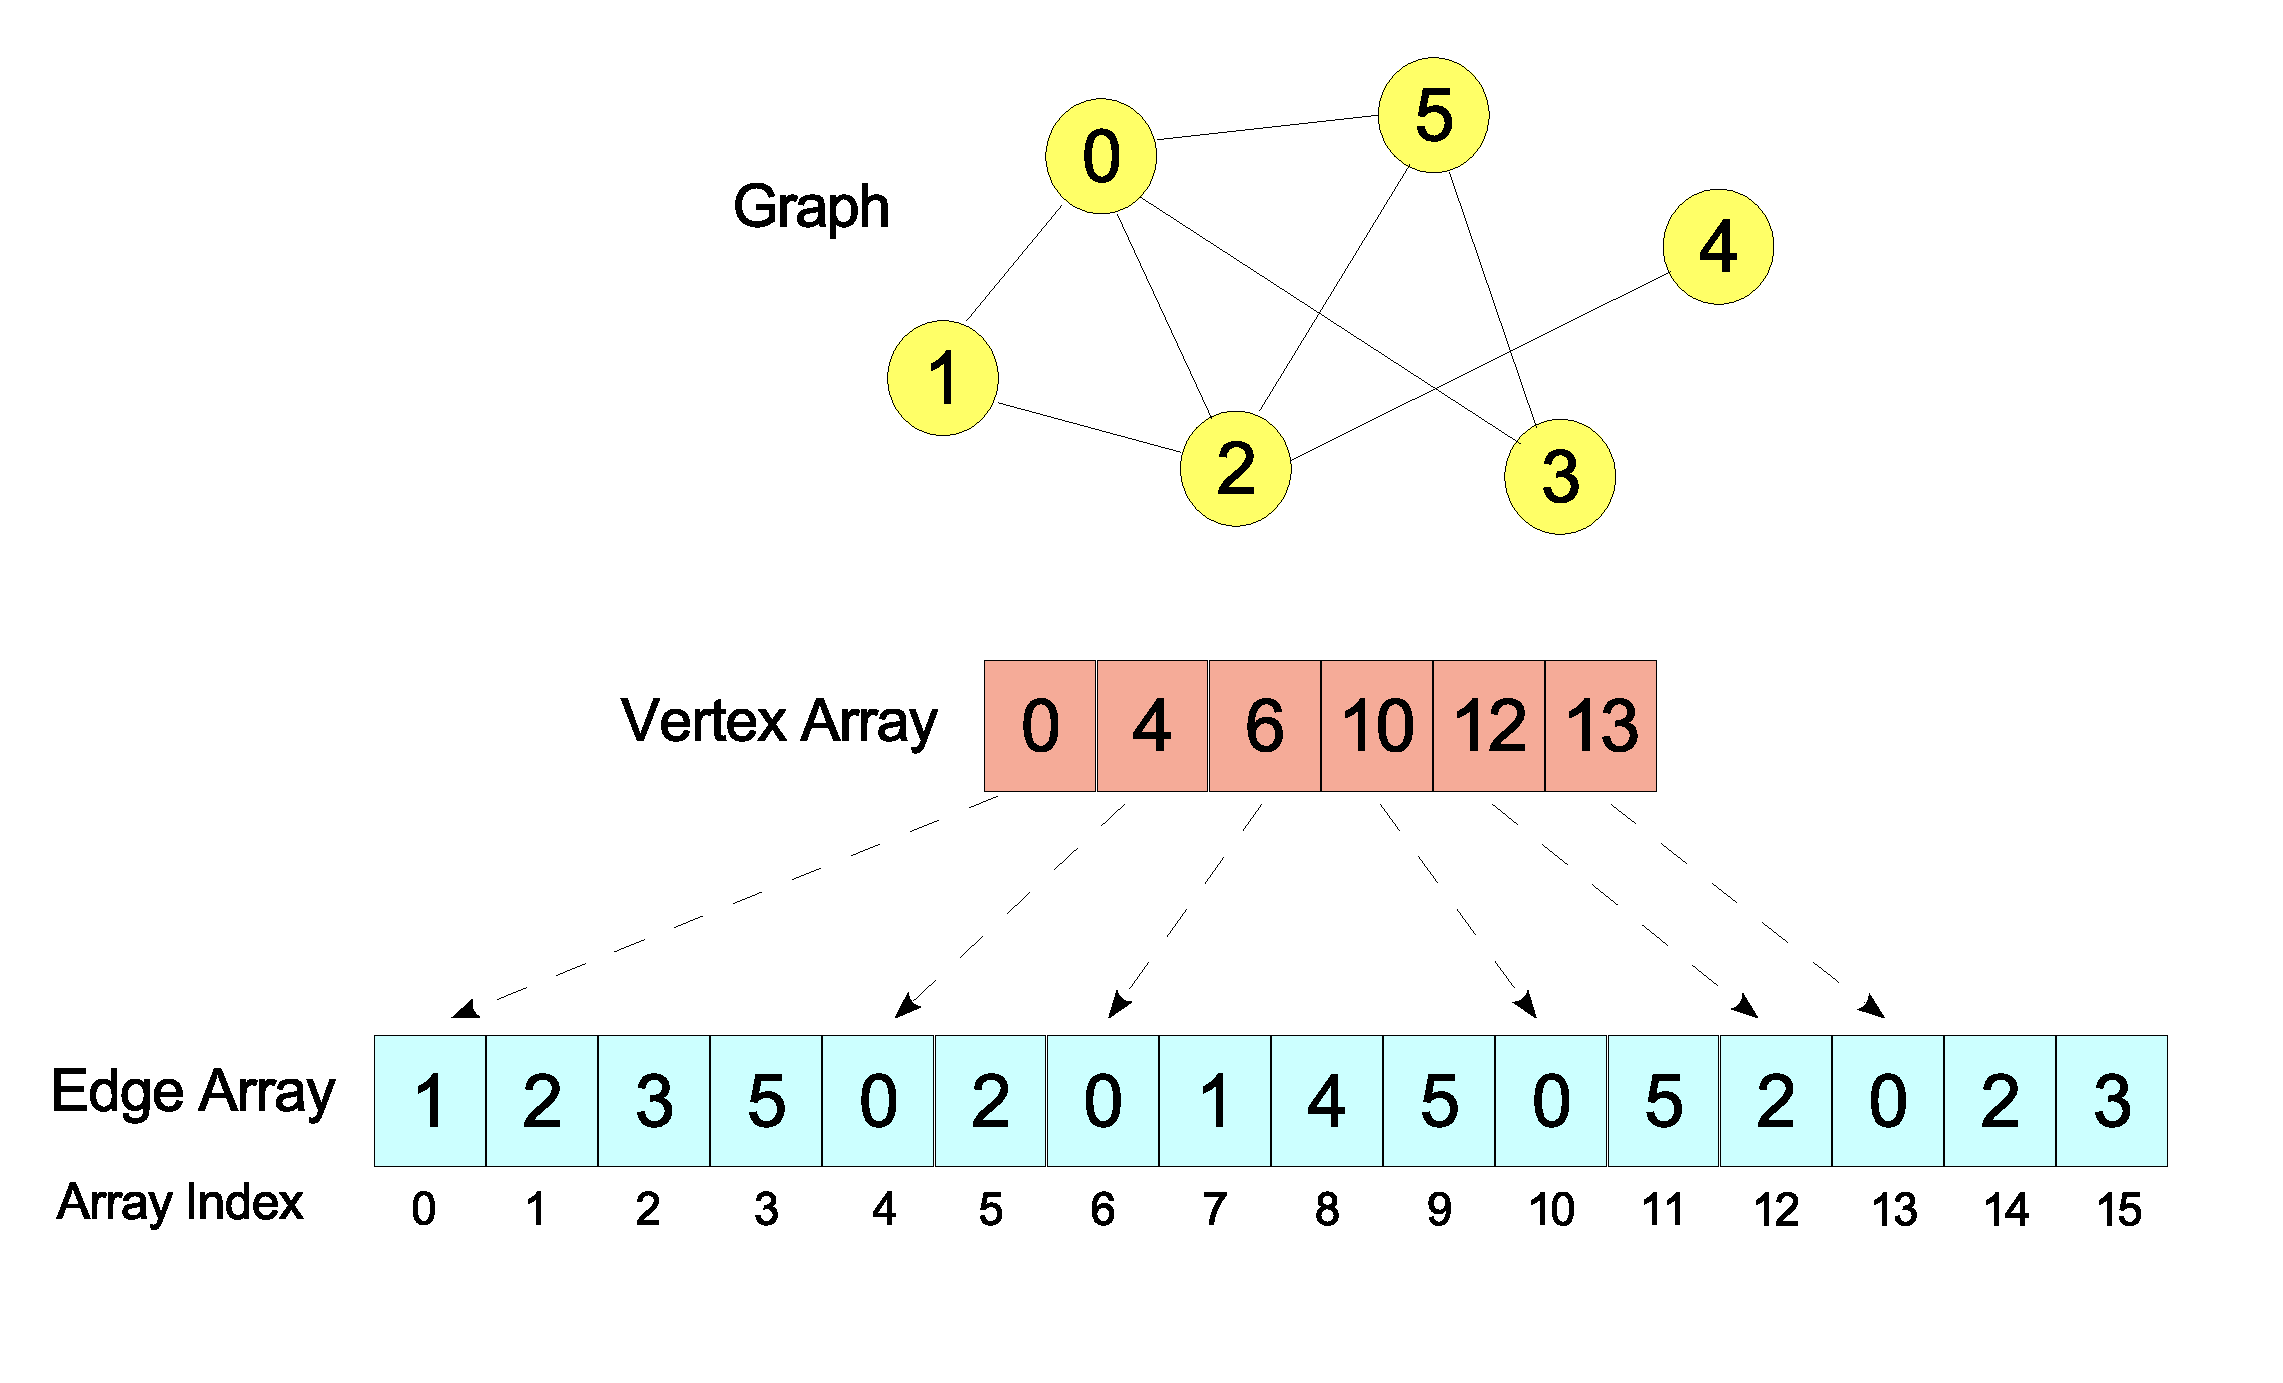
\includegraphics[scale=0.25]{implementation.eps}
\caption{{\bf The adjacency list data structure used in our implementation shown for a sample graph. Each element in the vertex array stores the index to the starting element of its neighbor list in the edge array.}}
\label{fig-implementation}
\end{figure}

